\documentclass{emulateapj}
\input sfrs.defs

\shorttitle{WISE SFRs}  
\shortauthors{Moustakas et~al.}

\begin{document}

\title{Calibration of Ultraviolet and Infrared Star Formation Rate
  Diagnostics from WISE Observations of Distant Galaxies}

\author{John Moustakas\altaffilmark{1} \etal}

\altaffiltext{1}{Center for Astrophysics and Space Sciences,
  University of California, 9500 Gilman Dr., La Jolla, CA 92093} 

\begin{abstract} 
This is abstract.
\end{abstract}

%\keywords{Surveys -- galaxies: distances and redshifts -- galaxies: evolution 
%-- galaxies: high-redshift -- cosmology: large-scale structure of universe} 

% Sec 1 - Introduction
\section{Introduction}\label{sec:intro}
My introduction is neat.

%\clearpage
% Sec 2 - the data
\section{Data}\label{sec:data}

We begin by selecting all galaxies in the SDSS/VAGC DR72 that overlap
the footprint of WISE observations released as part of their first
data release.  Maybe give the Galactic longitude limits?  [All
  magnitude limits are corrected for Galactic extinction using the
  \citet{schlegel98a} dust maps and the \citet{cardelli89a} Milky Way
  extinction law assuming $R_{V}=3.1$.]  The SDSS sample has $ugriz$
imaging and $3700-9200$~\AA{} spectrophotometry from the SDSS and is
flux-limited with $14.5<r<17.6$ and $0.01<z<0.25$.  Note that the
redshift cuts are very soft; roughly $98.9\%$ of the parent sample are
within these limits.  The parent sample has $521,604$ galaxies, of
which $200,862$ ($39\%$) are in the WISE footprint.  Next, we restrict
our sample to objects with MIS-depth GALEX imaging, i.e., FUV and NUV
exposure times $>1000$~s, leaving $48,694$ ($24\%$) galaxies.  We
require (Galactic extinction corrected) $\fuv=\nuv<23$ to ensure good
GALEX photometry.  Brighter than this limit GALEX is more than $80\%$
complete, while at fainter flux levels source confusion starts to
become important (wyder, schiminovich).  At the flux limit of our SDSS
sample objects with $\nuv-r>5.4$ will be excluded from our sample;
however, all of these should be passively evolving and would have to
have pathological amounts of dust extinction to be that red (calculate
how much!).  Our UV flux cuts leave $25,968$ ($74\%$) galaxies.

Next we apply flux cuts at $22$~\micron, which we need in order to be
able to estimate the infrared luminosities of the galaxies in our
sample.  In DR1 WISE is flux-limited above $6$~mJy ($5\sigma$), over
the whole survey region, and to fainter flux levels in areas with more
overlapping coverage \citep{wright10a}.  Therefore, we restrict our
sample to have $[22]<14.45$, including upper limits.  Need to talk
about which fluxes we use - profile, aperture, 2mass, etc.

\begin{figure}
\centering
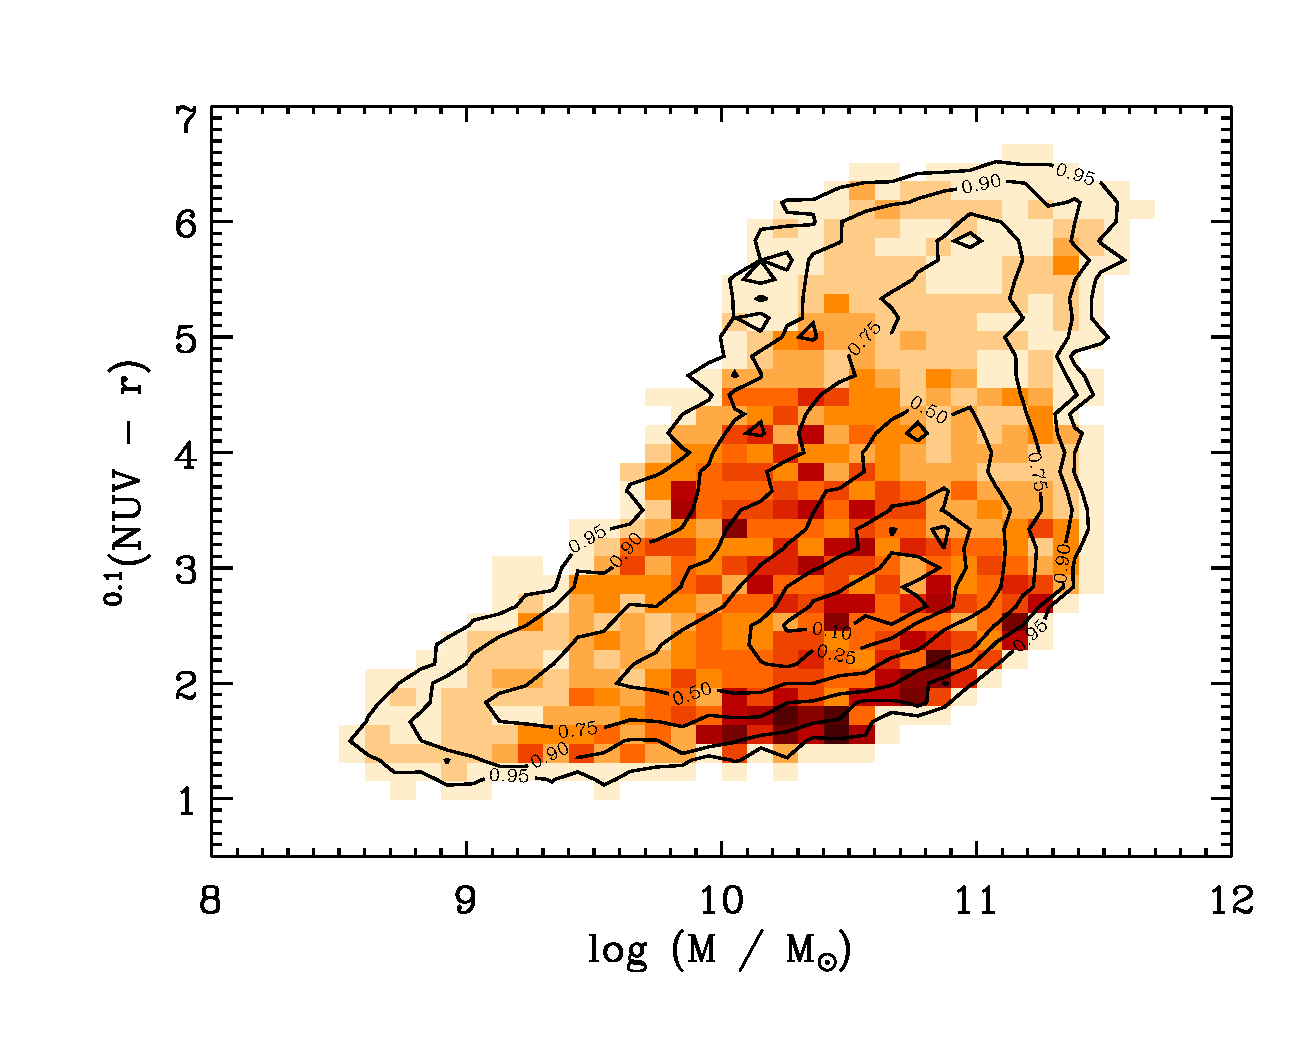
\includegraphics[scale=0.4]{nuvmr_mass}
\caption{UV-optical color-magnitude diagram. \label{fig:nuvmr}} 
\end{figure}
%\clearpage

%\clearpage
% Sec 3 - Results
\section{Results}\label{sec:results}
The results.

%\clearpage
% Sec 7 - Discussion
\section{Discussion \& Conclusions}\label{sec:discussion}  
This is my discussion and conclusions.

\acknowledgements
Thank people.  

This publication makes use of data products from the Wide-field
Infrared Survey Explorer, which is a joint project of the University
of California, Los Angeles, and the Jet Propulsion
Laboratory/California Institute of Technology, funded by the National
Aeronautics and Space Administration.

%% Bibliography

\bibliographystyle{apj}
\bibliography{/Users/ioannis/bibtex/im}

\end{document}

